\newcommand{\decktitle}{Programmiersprachen}

%%%%%%%%%%%%%%%%%%%%%%%%%%%%%%%%%%%%%%%%%%%%%%%%%
%
% DOCUMENT
%
%%%%%%%%%%%%%%%%%%%%%%%%%%%%%%%%%%%%%%%%%%%%%%%%%

\begin{frame}
    \subtitle{\decktitle}
    \titlepage
\end{frame}


\begin{frame}
    \frametitle{\textbf{Outline:}}
    \tableofcontents
\end{frame}

		
		
\section{Zweck von Programmiersprachen}		
    \begin{frame}{Programmiersprachen}
        Mithilfe von Computerprogrammen können komplexe wohldefinierte Problemstellungen (teil)automatisiert gelöst werden. Voraussetzung dafür ist, dass
        \begin{itemize}
            \item das Problem konkret beschrieben werden kann
            \item sich das Problem ihm Rahmen der Möglichkeiten einer Programmiersprache abbilden lässt
            \item es mindestens einen Lösungsweg gibt
            \item der Lösungsweg endlich ist
        \end{itemize}
    \end{frame}  
    
    \begin{frame}{Einordnung von Programmiersprachen}
        \begin{figure}
            \centering
            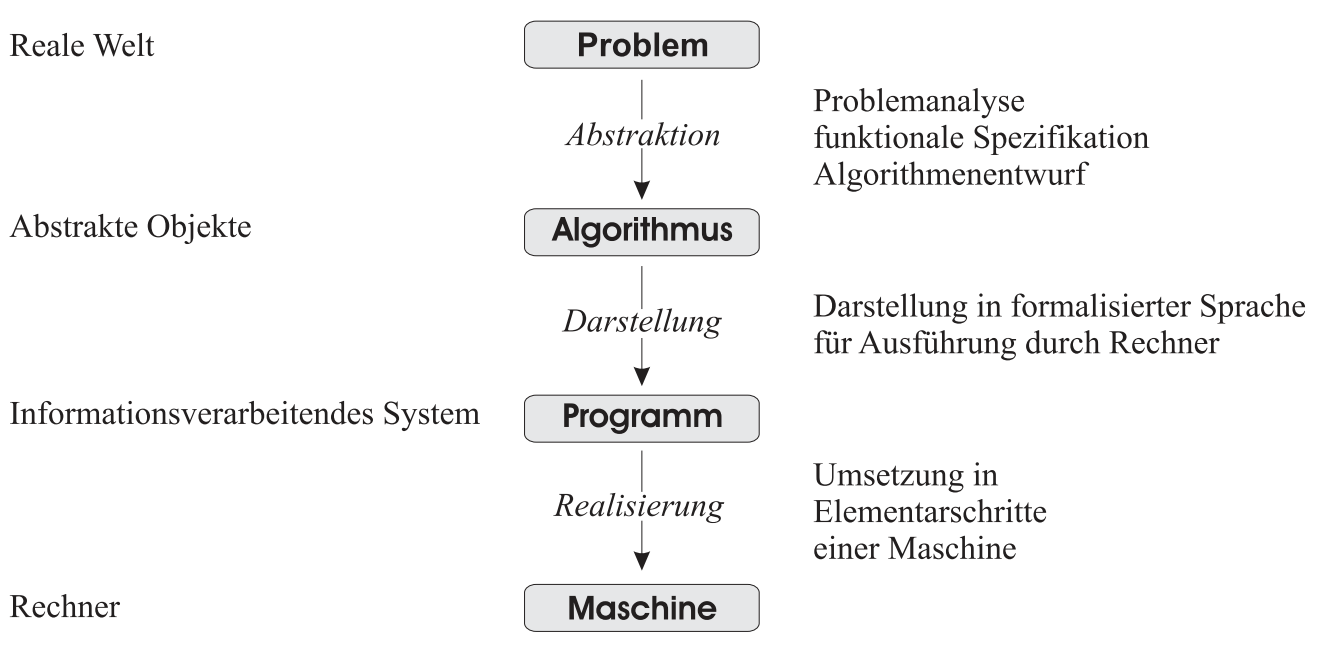
\includegraphics[width=\linewidth,height=0.5\textheight,keepaspectratio]{chapters/04_programming_languages/figures/problem2solution.png}
            \caption{Vorgehensweise zur Lösung von Problemen in der Informatik \cite{Muller2015}}
        \end{figure}
    \end{frame}
    
    \begin{frame}{Einordnung von Programmiersprachen}
        \begin{figure}
            \centering
            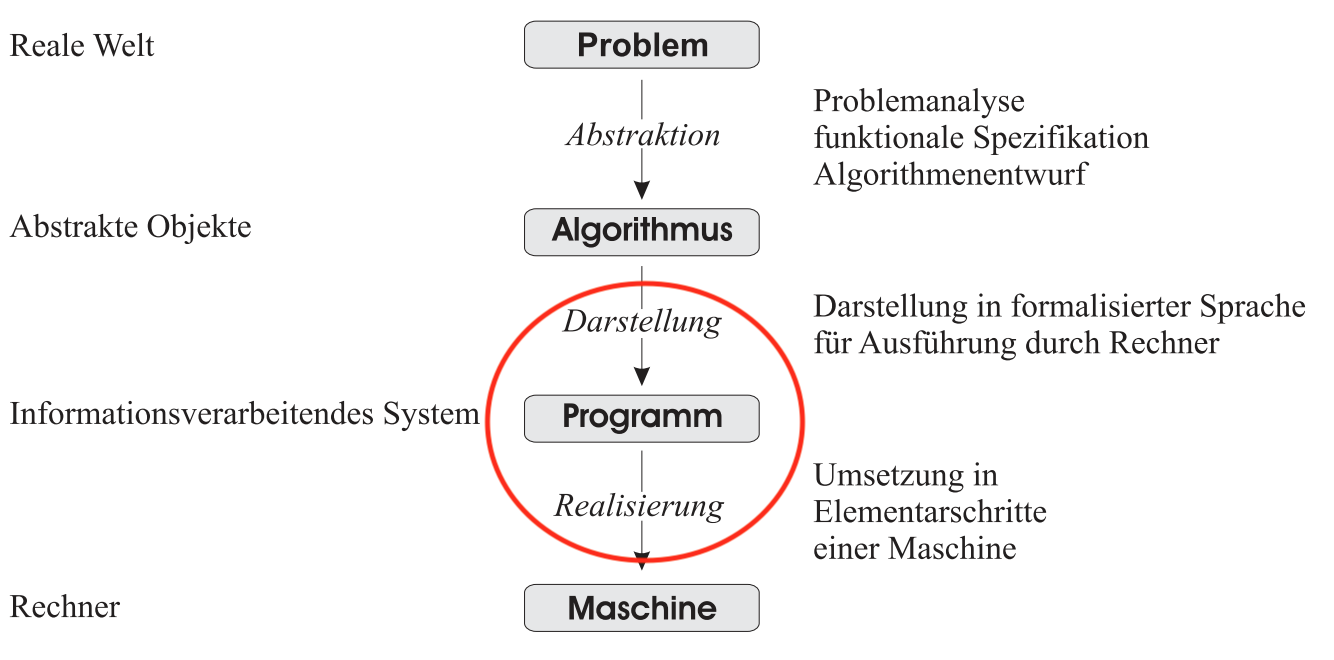
\includegraphics[width=\linewidth,height=0.5\textheight,keepaspectratio]{chapters/04_programming_languages/figures/problem2solution_marked.png}
            \caption{Vorgehensweise zur Lösung von Problemen in der Informatik \cite{Muller2015} (bearbeitet)}
        \end{figure}
    \end{frame}
    
    \begin{frame}{Zweck von Programmiersprachen}
        Programmiersprachen helfen also dabei, das Problem, welches zunächst abstrakt beschrieben wird, formal darzustellen und in eine Form zu übertragen, die für das Computersystem verarbeitbar ist.
    \end{frame}
    
    \begin{frame}{Einordnung von Programmiersprachen}
        \begin{figure}
            \centering
            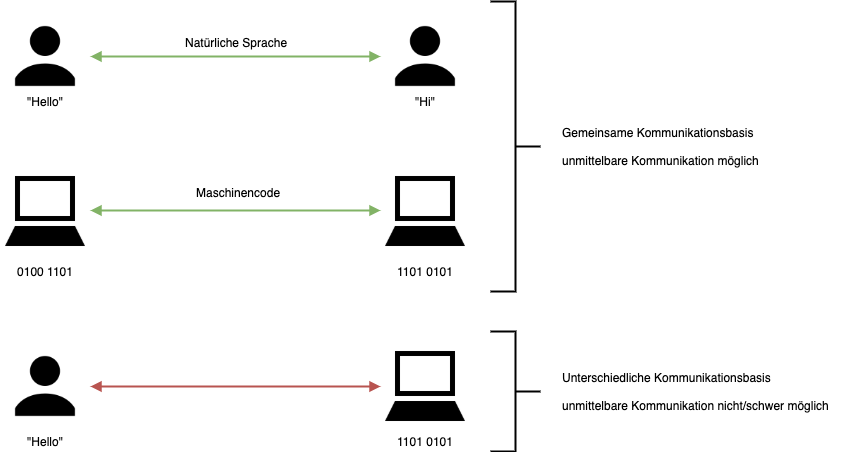
\includegraphics[width=\linewidth,height=0.5\textheight,keepaspectratio]{chapters/04_programming_languages/figures/communication_direct.png}
            \caption{Kommunikationswege zwischen Mensch und Computer (I)}
        \end{figure}
    \end{frame}
    
    \begin{frame}{Einordnung von Programmiersprachen}
        \begin{figure}
            \centering
            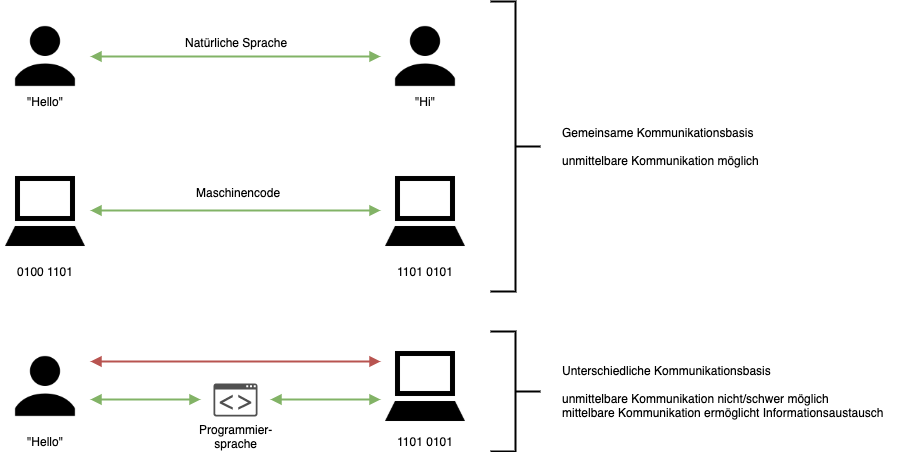
\includegraphics[width=\linewidth,height=0.5\textheight,keepaspectratio]{chapters/04_programming_languages/figures/communication_indirect.png}
            \caption{Kommunikationswege zwischen Mensch und Computer (II)}
        \end{figure}
    \end{frame}
    
\section{Vielfalt der Programmiersprachen}  

    \begin{frame}{Programmiersprachen}
        \begin{figure}
            \centering
            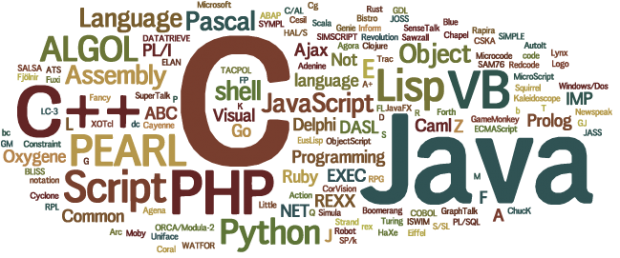
\includegraphics[width=\linewidth,height=0.5\textheight,keepaspectratio]{chapters/04_programming_languages/figures/languages.png}
            \caption{Word-Cloud zur Vielfalt an Programmiersprachen \cite{fig:programming_languages}}
        \end{figure}
    \end{frame}
    
    \begin{frame}{Beliebtheit von Programmiersprachen}
        \begin{figure}
            \centering
            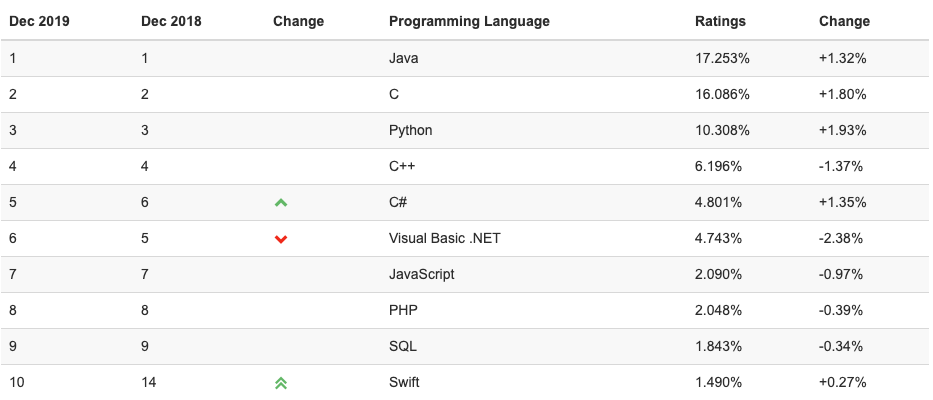
\includegraphics[width=\linewidth,height=0.5\textheight,keepaspectratio]{chapters/04_programming_languages/figures/tiobe_2019.png}
            \caption{TIOBE-Index zur Beliebtheit von Programmiersprachen 12/2019 \cite{fig:tiobe2019}}
        \end{figure}
        
        \begin{alertblock}{Hinweis}
        Der TIOBE-Index stellt keine wissenschaftliche Auswertung zur Beliebtheit von Programmiersprachen dar, die Ergebnisse sind lediglich auf Auswertungen von Suchanfragen gestützt. Dennoch bietet der Index einen groben Überblick.
        \end{alertblock}
    \end{frame}
    
    \begin{frame}{Beliebtheit von Programmiersprachen}
        \begin{figure}
            \centering
            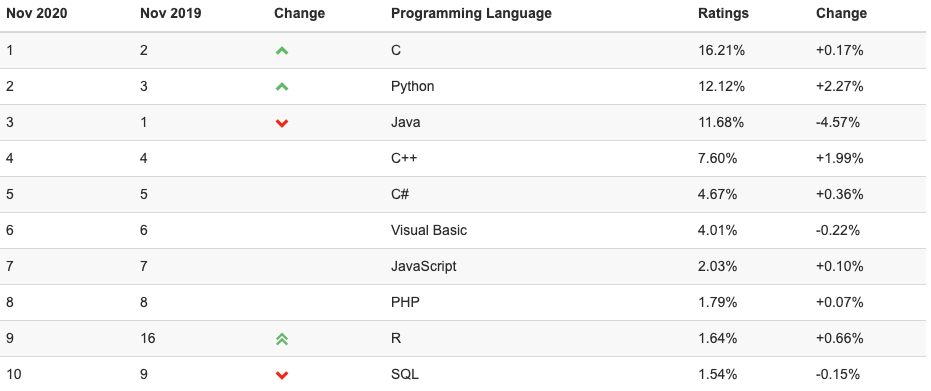
\includegraphics[width=\linewidth,height=0.5\textheight,keepaspectratio]{chapters/04_programming_languages/figures/tiobe_2020.png}
            \caption{TIOBE-Index zur Beliebtheit von Programmiersprachen 11/2020 \cite{fig:tiobe2019}}
        \end{figure}
        
    \end{frame}
    
    \begin{frame}{Beliebtheit von Programmiersprachen}
        \begin{figure}
            \centering
            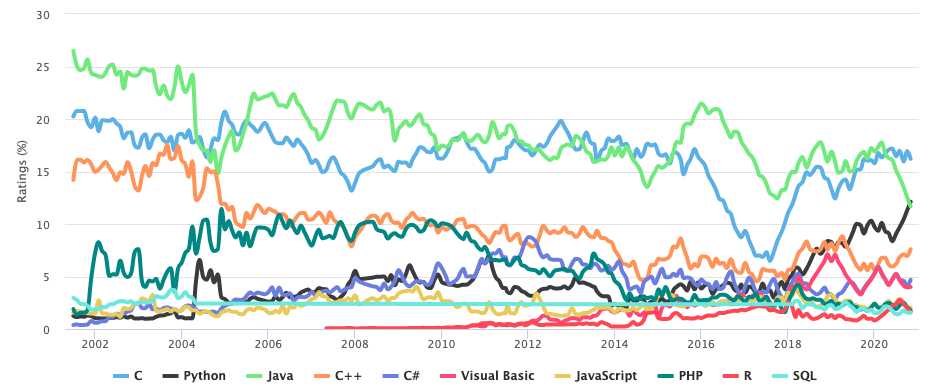
\includegraphics[width=\linewidth,height=0.5\textheight,keepaspectratio]{chapters/04_programming_languages/figures/tiobe_2002-2020.png}
            \caption{TIOBE-Index zur Beliebtheit von Programmiersprachen Juli 2001 - November 2020 \cite{fig:tiobe2001-2019}}
        \end{figure}
    \end{frame}
  
    \begin{frame}{Vielfältigkeit und Anzahl von Programmiersprachen}
        \begin{figure}
            \centering
            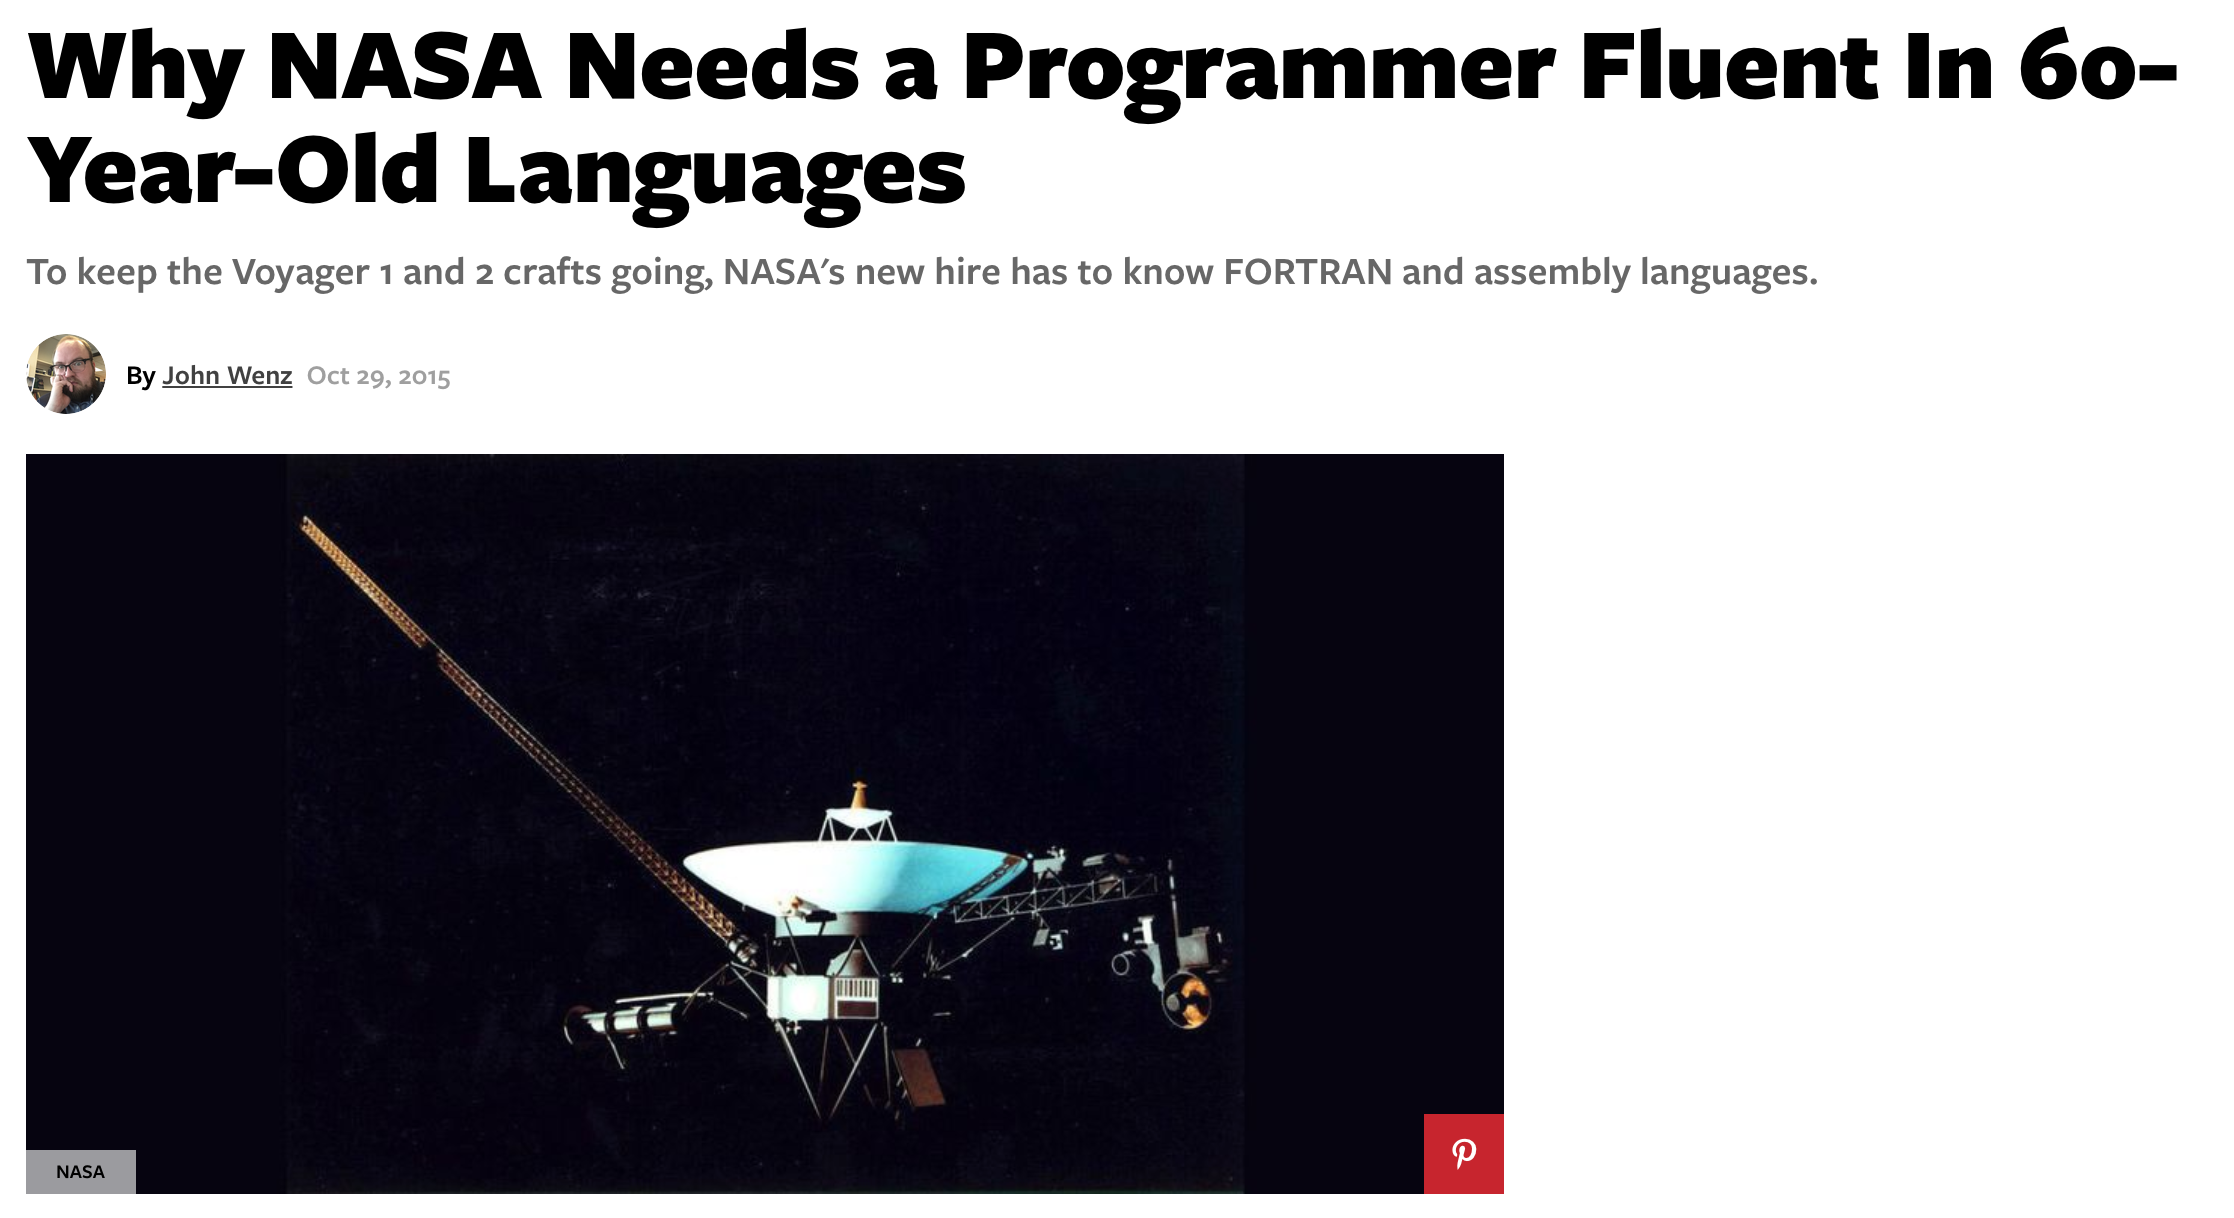
\includegraphics[width=\linewidth,height=0.5\textheight,keepaspectratio]{chapters/04_programming_languages/figures/voyager.png}
            \caption{Bericht über die Suche der NASA nach einem COBOL-Entwickler \cite{fig:voyager}}
            
        \note{
        1960er Jahre \\
        Fortran, Cobol, Assembler \\
        Radio-Übertragung, 17 Stunden
        }
        \end{figure}
        
    \end{frame}
    
    \begin{frame}{Frage 1: Was hat das mit Programmiersprachen zu tun?}
         \lstinputlisting[basicstyle=\tiny]{chapters/04_programming_languages/code/hello_world.spl}
    \end{frame}
    
    \begin{frame}{Frage 2: Was hat das mit Programmiersprachen zu tun?}
         \lstinputlisting[basicstyle=\tiny]{chapters/04_programming_languages/code/hello_world.tr}
    \end{frame}
    
    \begin{frame}{Frage 3: Was hat das mit Programmiersprachen zu tun?}
         \begin{figure}
            \centering
            
\includegraphics[width=\linewidth,height=0.5\textheight,keepaspectratio]{chapters/04_programming_languages/figures/hello_world_piet.jpg}
            \caption{\cite{fig:hello_world_piet}}
        \end{figure}
    \end{frame}
    
    \begin{frame}{Frage 4: Was hat das mit Programmiersprachen zu tun?}
         \lstinputlisting[basicstyle=\tiny]{chapters/04_programming_languages/code/hello_world.bf}
    \end{frame}
    
    
\section{Eigenschaften von Programmiersprachen (Gemeinsamkeiten)}
    \label{sec:properties}
    
    \begin{frame}{Eigenschaften}
        Alle Programmiersprachen müssen verschiedene Voraussetzungen erfüllen, damit es sich tatsächlich um eine Programmiersprache handelt. 
        
        \begin{alertblock}{Hinweis}
            Die im Folgenden aufgeführten Eigenschaften stellen lediglich die "Mindestvoraussetzungen" von Programmiersprachen dar. Die Programmiersprachen besitzen darüber hinaus noch viele weitere Eigenschaften, die sich jedoch unterscheiden können bzw. nicht zwingend in jeder Programmiersprache vorhanden sein müssen.
        \end{alertblock}
    \end{frame}
     
    \begin{frame}{Eingabe \& Ausgabe}
        Jede Programmiersprache muss \textbf{Eingaben} verarbeiten können (Informationsquelle). Dabei spielt es keine Rolle, ob die Eingabe durch eine manuelle Nutzereingabe (z.B. Text durch Tastatur/Maus, Spracheingabe, Dokumentenscan, ...) oder durch automatisiertes Einlesen von Daten (z.B. Datenbank, Datei, Programmierschnittstelle, ...)  erfolgt. \\~\
        
        Ebenso muss die \textbf{Ausgabe} von Informationen möglich sein, um dem Nutzer oder einem anderen System die Ergebnisse zur Verfügung zu stellen (Informationssenke). Auch hierfür gibt es genauso wie bei der Eingabe verschiedene Möglichkeiten (z.B. Ausgabe am Bildschirm, Audioausgabe, Datenbank, ...)  \\~\
        
        Auf welche Art und Weise und in welchem Format die Ein- und Ausgabe erfolgt ist jeweils abhängig vom Anwendungsfall und der Umsetzung im Programm und ist daher nicht vorgegeben.
        
        \note{
        Eingabe: Quelle, verschiedene Quellen \\
        Ausgabe: Ziel / Senke, verschiedene Ziele \\
        
        z.B. Sprachassistenten, Touchscreen, ... \\
        Quelle / Ziel abhängig von Implementierung
        }
    \end{frame}
    
    
    \begin{frame}{Deklaration von Variablen}
        Um Informationen innerhalb eines Programms verarbeiten zu können, müssen die Daten während der Verarbeitung zwischengespeichert werden. Hierzu werden Variablen genutzt, um Informationen referenzieren (darauf zugreifen) zu können. \\~\
        
        \begin{block}{Variable}
            Speichereinheit zur Aufnahme, Zwischenspeicherung und Modifikation von Daten(werten)
        \end{block}
        
        \begin{block}{Deklaration}
            Zuweisung / Zuordnung eines bestimmten Werts zu einer bestimmten Variablen (zu einem bestimmten Variablennamen)
        \end{block}
        
        \note{
            Zwischenspeicherung von Werten \\
            Speicherung in Variablen
        }
    \end{frame}
    
    \begin{frame}{Mathematische Grundoperationen}
        Wenn Informationen nicht nur (zwischen)gespeichert, sondern auch verarbeitet werden sollen, sind mathematische Grundoperationen unabdingbar. Auf Maschinencode-Ebene werden beinahe sämtliche Operationen durch Addition ausgeführt. Aber auch in höheren Programmiersprachen sind keine Berechnungen ohne mathematische Standardfunktionen möglich.
        
        \note{
            Verarbeitung von Werten / Variablen
        }
    \end{frame}
    
    \begin{frame}{Zeichenkettenverarbeitung}
        Während mathematische Grundoperationen zur Verarbeitung von Zahlen benötigt werden, müssen auch Funktionen zur Verarbeitung und Speicherung von Zeichenketten (Strings) bereitstehen. \\~\
        
        \begin{block}{String}
            Ein String (Zeichenkette) repräsentiert in der Programmierung Text. Dazu können Buchstaben, Sonderzeichen, Satzzeichen und Steuerzeichen gehören
        \end{block}
        
        \note{
            Zeichenketten = Strings (Buchstaben, Ziffern, Sonderzeichen, Satzzeichen, Steuerzeichen)
        }
    \end{frame}
    
    \begin{frame}{Steueranweisungen}
        Zu den Steueranweisungen gehören alle Befehle und Operationen, die den Ablauf eines Programms beschreiben und beeinflussen. \\~\
        
        Dazu können etwa Schleifen, bedingte Anweisungen, Funktionen / Prozeduren, und andere Sprachkonstrukte gehören.
        
        \note{
            Steueranweisungen = beeinflussen Ablauf eines Programms
            
        }
    \end{frame}
    
    \begin{frame}{Zusammenfassung}
        Zu den Eigenschaften jeder Programmiersprache gehören folgende Grundfunktionalitäten:
        
        \begin{itemize}
            \item Ein- und Ausgabe von Informationen
            \item Deklaration von Variablen und Verarbeitung deren Werten
            \item Mathematische Grundoperationen zur Verarbeitung von Zahlenwerten
            \item Zeichenkettenverarbeitung zur Verarbeitung von Strings
            \item Steueranweisungen zur Programmablaufbeschreibung
        \end{itemize}
    \end{frame}
        
\section{Einordnung und Gruppierung von Programmiersprachen (Unterschiede)}
    
    \begin{frame}{Einordnung von Programmiersprachen}
        Programmiersprachen können aufgrund unterschiedlicher Konzepte, Eigenschaften und Merkmale unterschieden und so in diverse Gruppen eingeteilt werden. In manchen Bereichen ist eine klare oder eindeutige Zuordnung einer bestimmten Programmiersprache zu einer Gruppe nicht oder nur schwer möglich. \\~\
        
        Im Folgenden werden die wichtigsten Merkmale, anhand deren die Programmiersprachen unterschieden werden können, dargestellt. Die Aufzählung hat nicht den Anspruch der Vollständigkeit, da die Unterschiede auch subjektiv erhoben werden können.
        
        \note{
            unterschiedl. Konzepte, Eigenschaften, Merkmale \\
            daher unterschiedliche Gruppen von Sprachen \\
            
            nicht immer eindeutige Zuordnung einer Sprache möglich 
        }
    \end{frame}
    
        \subsection{Programmierparadigmen}
        
            \begin{frame}{Programmierparadigmen}
                Programmiersprachen können nach unterschiedlichen Paradigmen bzw. Mustern unterteilt werden. Ein Programmierparadigma beschreibt dabei einen bestimmten Stil, an dem sich die Programmierung, Umsetzung der Lösung und Implementierung des Codes orientiert. \\~\
                
                Meist werden unterschiedliche Programmiersprachen einem Programmierparadigma zugeordnet, in manchen Fällen ist das Paradigma von der Sprache aber nicht fest vorgegeben, sodass dem Entwickler die Entscheidung für ein Paradigma überlassen ist. \\~\
                
                Programmiersprachen können auch nach mehreren Programmierparadigmen gestaltet sein.
                
                \note{
                   Pradigmen = Muster, das den Programmierstil beschreibt, an dem sich Programmierung, Umsetzung und Implementierung orientiert \\
                   versch. Vorgehen \\
                   nicht formal, sondern methodisch
                   
                }
            \end{frame}
            
            \begin{frame}{Programmierparadigmen}
                \begin{figure}
                    \centering
                    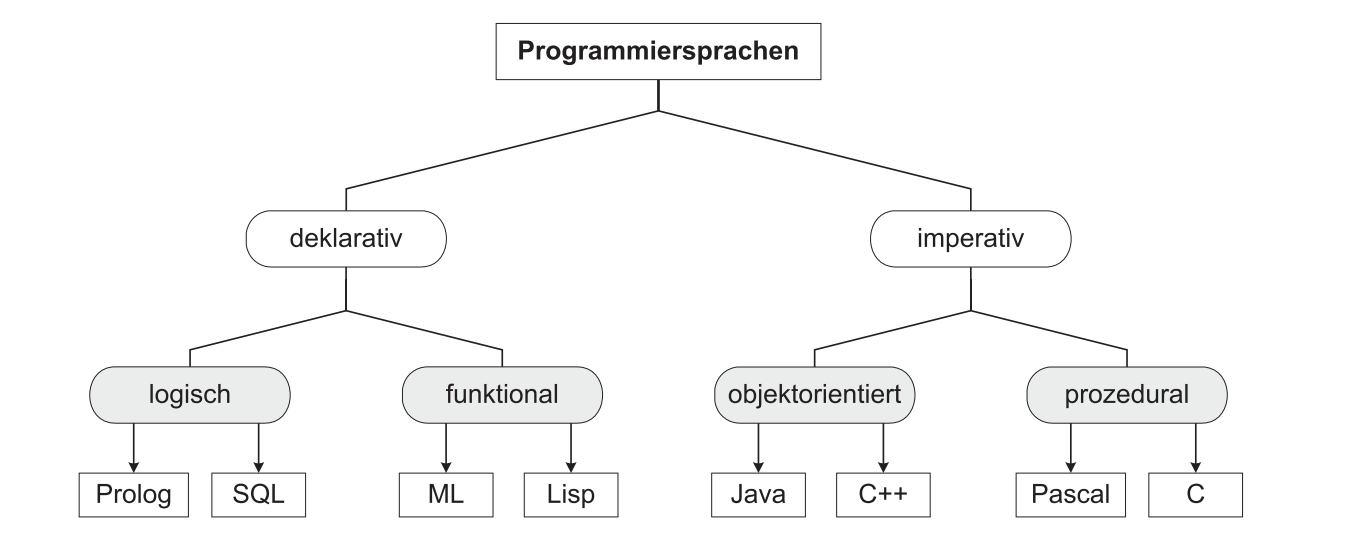
\includegraphics[width=\linewidth,height=0.5\textheight,keepaspectratio]{chapters/04_programming_languages/figures/paradigms/paradigms.png}
                    \caption{Gliederung der Programmiersprachen nach unterschiedlichen Paradigmen \cite{Muller2015}}
                \end{figure}   
            \end{frame}
            
            \begin{frame}{Programmierparadigmen: Imperativ (I)}
                \begin{figure}
                    \centering
                    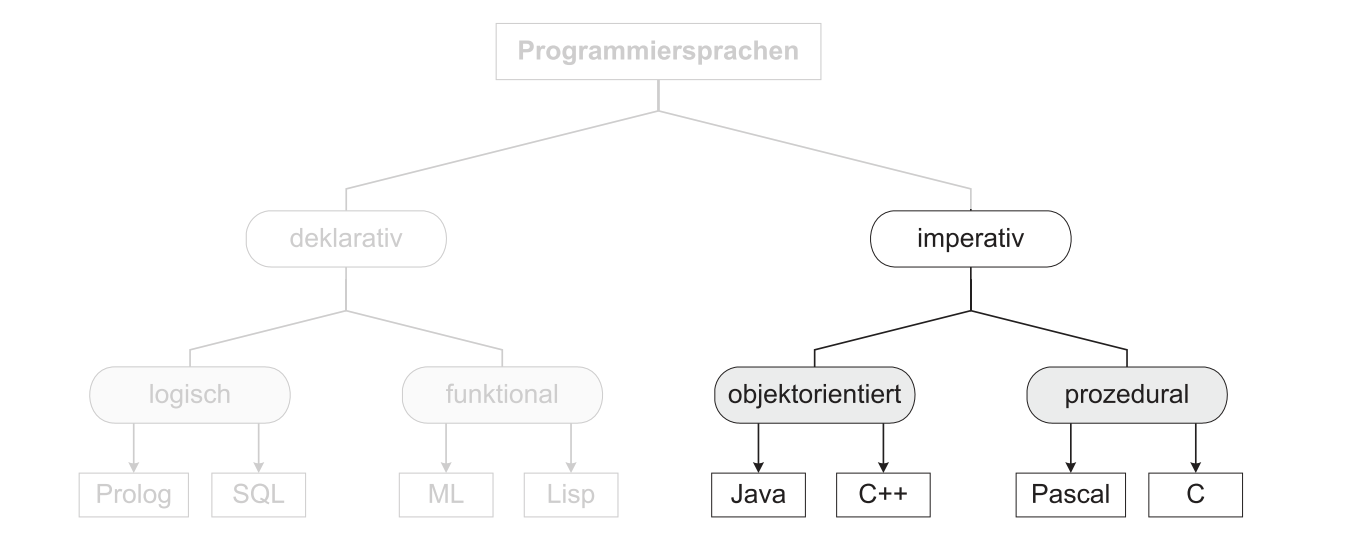
\includegraphics[width=\linewidth,height=0.5\textheight,keepaspectratio]{chapters/04_programming_languages/figures/paradigms/imperative.png}
                    \caption{Gliederung der Programmiersprachen nach unterschiedlichen Paradigmen \cite{Muller2015} (bearbeitet)}
                \end{figure}   
            \end{frame}
            
            \begin{frame}{Programmierparadigmen: Imperativ (II)}
                Bei der \textit{imperativen Programmierung} beschreibt der Programmierer, was der Reihe nach ausgeführt werden soll. Er ist also sowohl für die zugrundeliegende Funktionalität als auch für die ordnungsgemäße Reihenfolge dieser Anweisungen zuständig. \\~\
                
                Die imperative Programmierung stellt das älteste und weitverbreitetste Paradigma dar, da es große Ähnlichkeiten zum menschl. Denkprozess aufweist.\\~\
                
                \begin{block}{Imperative Programmierung}
                    Ursprung: \textit{imperare} (lat.): \textit{'anordnen', 'befehlen'} \\
                    Der Programmierer beschreibt, \textbf{wie} eine Lösung zu einem bestimmten Problem ermittelt wird.
               \end{block}
               
               \note{
                   was wird der Reihe nach ausgeführt \\
                   konkrete Befehle an den Computer, Step by Step\\
                   Programmierer ist für zugrundeliegende Funktionalität als auch für Reihenfolge der Anweisungen zuständig \\
                   einfach zu verstehen
                }
            \end{frame}
            
            \begin{frame}{Programmierparadigmen: Imperativ (III)}
                Häufig wird innerhalb der imperativen Programmierung zwischen zwei weiteren (konträren) Paradigmen unterschieden: \\~\ 
                
                \begin{columns}[T]
                    \begin{column}{0.5\textwidth}
                        \textbf{Prozedural}
                        \begin{itemize}
                            \item Programmablauf kann in Teilprobleme zerlegt werden
                            \item Wichtig zur Übersichtlichkeit, Wartbarkeit und Vermeidung von Redundanz
                            \item Daten und Funktionen haben keinen definierten Zusammenhalt
                        \end{itemize}
                    \end{column}
                    
                    \begin{column}{0.5\textwidth}
                        \textbf{Objektorientiert}      
                        \begin{itemize}
                            \item Funktionalitäten werden innerhalb von Klassen nach Zuständigkeit getrennt
                            \item Über einfache Datenstrukturen hinausgehende Abstraktion der Daten und Funktionalität 
                            \item Daten und Funktionen werden in Klassen / Objekten zusammengefasst
                        \end{itemize}
                    \end{column}
                \end{columns}
                
                \note{
                   Unterscheidung zwischen Prozedural und Objektorientiert
                }
            \end{frame}
            
            \begin{frame}{Programmierparadigmen: Deklarativ (I)}
                \begin{figure}
                    \centering
                    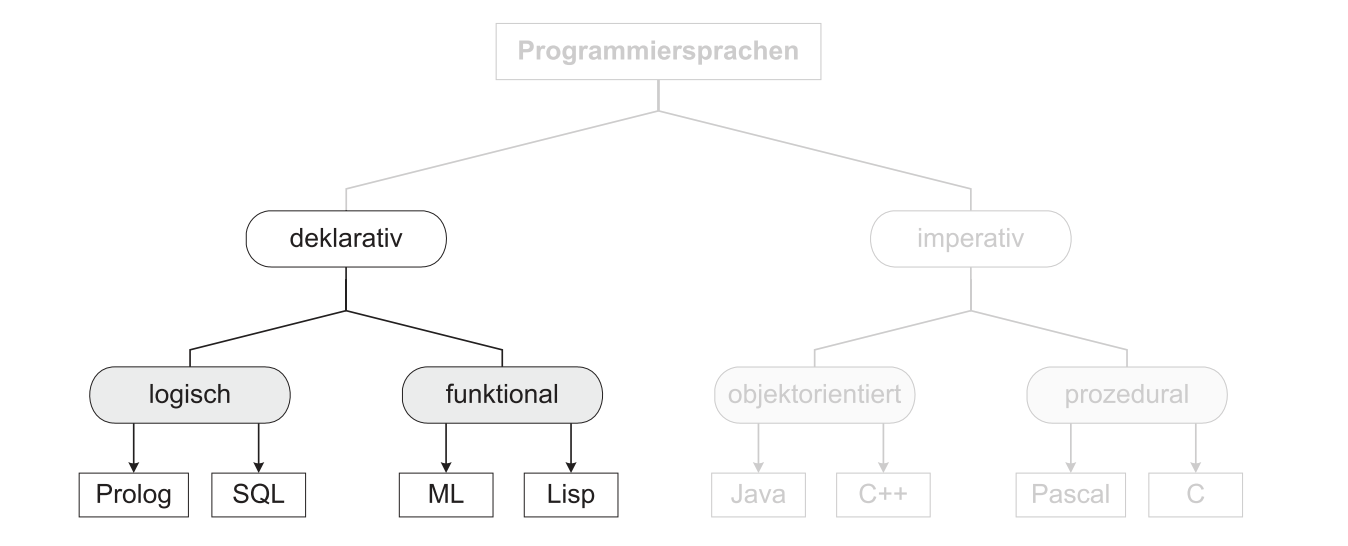
\includegraphics[width=\linewidth,height=0.5\textheight,keepaspectratio]{chapters/04_programming_languages/figures/paradigms/declarative.png}
                    \caption{Gliederung der Programmiersprachen nach unterschiedlichen Paradigmen \cite{Muller2015} (bearbeitet)}
                \end{figure}   
            \end{frame}
            
            \begin{frame}{Programmierparadigmen: Deklarativ (II)}
                Bei der \textit{deklarativen Programmierung} beschreibt der Programmierer nicht, was der Reihe nach ausgeführt werden soll, sondern \textit{was} berechnet werden soll. Dadurch steht hier vielmehr die Beschreibung des Problems als die explizite Beschreibung des Lösungswegs im Vordergrund. \\~\
                
                Im Gegensatz zur imperativen Programmierung lassen sich hier Arbeits- und Steuermechanismen trennen, sodass dieses Paradigma rechnerunabhängig ist. \\~\
                
                \begin{block}{Deklarative Programmierung}
                    Ursprung: \textit{declarar} (lat.): \textit{'erklären'} \\
                    Der Programmierer beschreibt, \textbf{was} berechnet werden soll und nicht, wie der entsprechende Rechenweg dafür aussieht.
               \end{block}
               
               \note{
                   Grundsätzlich anders als imperative Programmierung \\ 
                   Beschreibung \textbf{was} berechnet werden soll, nicht wie \\ 
                   Beschreibung des Problems ist wichtig, nicht der Lösungsweg \\
                   Trennung von Arbeits- und Steuermechanismen
                }
            \end{frame}
            
            \begin{frame}{Programmierparadigmen: Imperativ vs. Deklarativ}
            
                Beispiel: Durchsuche Bibliothekskatalog nach Büchern mit dem Titel "Programmierung" \footnote{angelehnt an \cite{leimeister}}
                
                \begin{exampleblock}{Beispiel: Imperative Programmierung}
                    \begin{enumerate}
                        \item Nimm Buch
                        \item Prüfe, ob Titel = "Programmierung"
                        \item Falls JA, notiere Autor
                        \item Prüfe, ob letztes Buch
                        \item Falls NEIN, gehe zu (1)
                        \item Falls JA \textrightarrow Ende
                    \end{enumerate}
                \end{exampleblock}
                
                \begin{exampleblock}{Beispiel: Deklarative Programmierung}
                    \begin{enumerate}
                        \item Suche alle Bücher, für die gilt (Titel = "Programmierung")
                    \end{enumerate}
                \end{exampleblock}
            \end{frame}
        
        \subsection{Maschinennähe}
            \begin{frame}{Maschinennähe}
                Beschreibt den Abstraktionsgrad bzw. die Nähe der Programmiersprache zum darunterliegenden System \\~\
                
                Maschinennahe Sprachen ("Low-Level Sprachen") bieten mehr Kontrolle und können tiefer in Systemfunktionalitäten eingreifen, sind aber meist auch komplexer und schwerer zu beherrschen als höhere Sprachen ("High-Level Sprachen") \\~\
                
                \begin{columns}[T]
                    \begin{column}{0.5\textwidth}
                        \textbf{Low-Level Sprachen}
                        
                        \begin{itemize}
                            \item Geringer oder kein Abstraktionsgrad
                            \item Direkte Speicherzugriffe, Kernelzugriffe, ... möglich
                            \item Mehr Kontrolle, höhere Komplexität
                            \item Beispiele: Maschinencode, Algol, Assembler, C
                        \end{itemize}
                    \end{column}
                    \begin{column}{0.5\textwidth}
                        \textbf{High-Level Sprachen}
                        
                        \begin{itemize}
                            \item Hoher Abstraktionsgrad
                            \item Keine direkten Speicherzugriffe, Kernelzugriffe, ... möglich
                            \item Weniger Kontrolle, geringere Komplexität
                            \item Beispiele: Java, Python, C++
                        \end{itemize}
                    \end{column}
                \end{columns}
                
                \note{
                   Grad der Abstraktion \\
                   Mehr Kontrolle, tiefe Systemeingriffe vs. Bedienungsfreundlichkeit, flache Lernkurve
                }
            \end{frame}
        
        \subsection{Computersprachen}
            \begin{frame}{Computersprachen}
                Nicht alle Sprachen, die häufig als "Programmiersprachen" bezeichnet werden, sind auch tatsächlich Programmiersprachen, da sie beispielsweise nicht alle Eigenschaften einer Programmiersprache erfüllen (siehe Abs. \ref{sec:properties}). Daher können Sprachen auch entsprechend ihres Zwecks untergliedert werden:
                
                \begin{itemize}
                    \item \textbf{Programmiersprache}: Kann komplexe Programmabläufe darstellen, besitzt alle beschriebenen Eigenschaften einer Programmiersprache (Beispiel: Python, Java, C)
                    \item \textbf{Datenbanksprache}: Wird zur Kommunikation mit einem Datenbanksystem verwendet (Beispiel: SQL)
                    \item \textbf{Auszeichnungssprache}: Beschreibt den Aufbau und die Struktur von Dokumenten (Beispiel: HTML, XML)
                    \item \textbf{Stylesheet-Sprache}: Beschreibt das Erscheinungsbild von Dokumenten unabhängig vom Inhalt (Beispiel: CSS)
                \end{itemize}
                
            
            \end{frame}

        \subsection{Typisierung}
            \begin{frame}{Typisierung / Typsysteme}
                In jeder Programmiersprache können Variablen erzeugt werden, denen unterschiedliche Arten von Werten (\textbf{Datentypen}) zugewiesen werden können. Dazu zählen bspw. Zahlen (Ganzzahlen, Fließkommazahlen), Zeichenketten (Strings) und Wahrheitswerte. Die Typisierung einer Programmiersprache dient zur korrekten Verwendung dieser Datentypen. \\~\
                
                Der Umgang mit den Datentypen kann sich zwischen den Programmiersprachen unterscheiden.
                
                \note{
                   Variablen können versch. Werte beinhalten \\
                   Ganzzahlen , Fließkommazahlen, Strings, Warhheitswerte \\
                   korrekte Verwendung der Datentypen
                }
            \end{frame}
            
            \begin{frame}{Typisierung / Typsysteme: Typenlose Sprachen}
                Manche Sprachen sind typenlose Sprachen. Derartige Programmiersprachen verfügen über keine differenzierten Datentypen. Das ist für den Entwickler einerseits sehr bequem, da er sich nicht um die entsprechenden Datentypen kümmern muss, führt aber auch schnell zu Fehlern, die aufgrund fehlender Typbezeichnungen manchmal nur schwer festzustellen und zu finden sind.  \\~\
                
                Beispiel: Assembler
                
                \note{
                   Verfügen über keine differenzierten Datentypen \\
                   bequem aber fehleranfällig
                }
                
            \end{frame}
            
            \begin{frame}{Typisierung / Typsysteme: Typisierte Sprachen}
                Die meisten Programmiersprachen sind typisiert, d.h. alle Variablen besitzen jederzeit einen bestimmten Datentyp. \\~\
                
                Typsysteme können weiter klassifiziert werden:
                \begin{itemize}
                    \item Statische vs. dynamische Typisierung: Typprüfungen finden zur Übersetzungszeit (statisch) oder zur Laufzeit (dynamisch) statt
                    \item Explizite vs. implizite Typisierung: Datentypen werden explizit genannt oder implizit ermittelt
                    \item Starke vs. schwache Typisierung: Verlustbehaftete Typumwandlungen können nicht (stark) / können (schwach) durchgeführt werden
                \end{itemize}
                
                \note{
                   alle Variablen besitzen einen Datentyp \\
                   statisch / dynamisch: Prüfung zur Runtime vs Compiletime \\
                   explizit / implizit \\
                   stark vs. schwach: Verlustbehaftete Umwandlung möglich
                   
                   
                }
            \end{frame}
            
            \begin{frame}{Anwendungsbereich}
                Manche Programmiersprachen werden nur domänenspezifisch eingesetzt, andere sind universell einsetzbar \footnote{Fettgedruckte Sprachen sind explizit für den jeweiligen Einsatzbereich entwickelt und werden ausschließlich dort verwendet}.
                
                \begin{itemize}
                    \item Websprachen (Serverseitig): \textbf{PHP}, \textbf{Ruby}, \textbf{node.js}, Python, Java
                    \item Websprachen (Clientseitig): \textbf{JavaScript}
                    \item Mobile Applications: \textbf{Kotlin} / Java (Android), \textbf{Swift} / Objective-C (iOS)
                    \item Business Applications: Java, C++, C\#
                    \item Datenbanken: \textbf{SQL}
                \end{itemize}
            \end{frame}
            
            
            \subsection{Appendix}
            
            \begin{frame}{Antwort 1: Was hat das mit Programmiersprachen zu tun?}

                \begin{columns}
                    \begin{column}{0.4\linewidth}
                        \begin{figure}
                            \centering
                            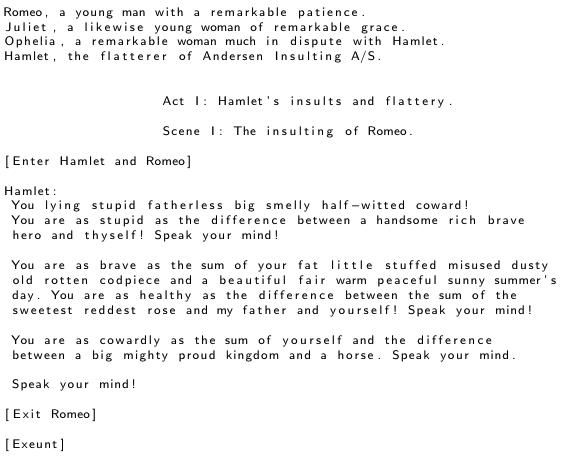
\includegraphics[width=\linewidth,height=0.5\textheight,keepaspectratio]{chapters/04_programming_languages/figures/shakespeare_code.png}
                        \end{figure}
                    \end{column}
                    \begin{column}{0.6\linewidth}
                        \begin{figure}
                            \centering
                            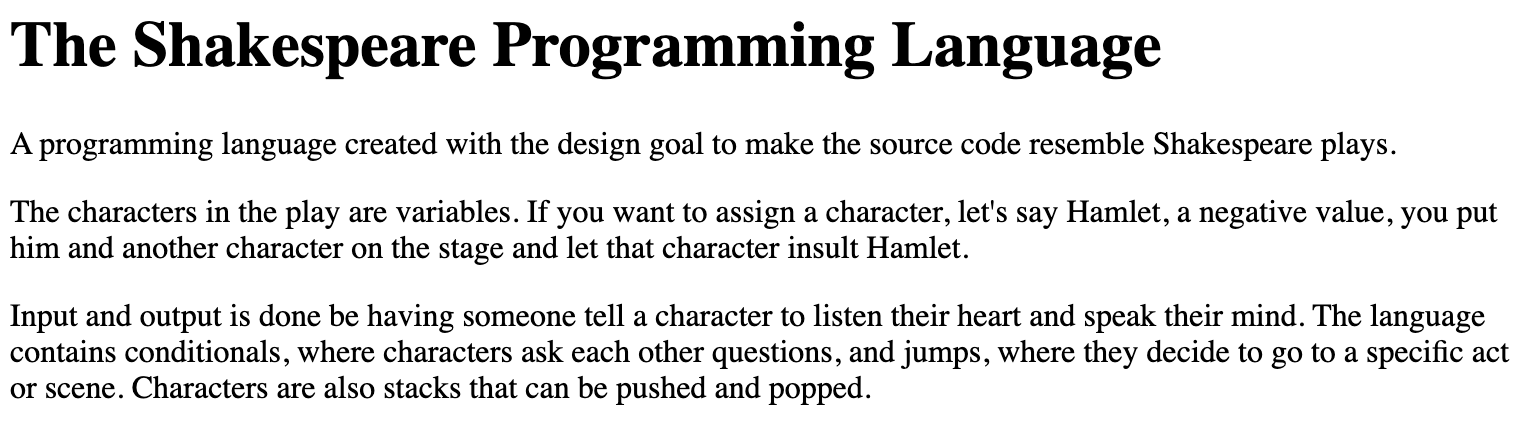
\includegraphics[width=\linewidth,height=0.5\textheight,keepaspectratio]{chapters/04_programming_languages/figures/shakespeare.png}
                            \caption{The Shakespeare Programming Language \cite{shakespeare_pl}}
                        \end{figure}
                    \end{column}
                \end{columns}
                \note{
                Titel: frei gewählt, keine Bedeutung \\
                Charaktere: Zu Beginn müssen die Personen festgelegt werden (Variablen) \\
                Akte \& Szenen: Sprungmarken, ansonsten nicht berücksichtigt \\
                Enter, Exit \& Exeunt: Charaktere müssen auf der Bühne stehen \\
                Dialog: Anweisungen, Eingabe, Ausgabe, Kontrollanweisungen \\
                Literale: negative Konnotation (-1), neutral (0), positive Konnotation (+1)
                }
                
            \end{frame}
            
             \begin{frame}{Antwort 2: Was hat das mit Programmiersprachen zu tun?}
                \begin{columns}
                    \begin{column}{0.4\linewidth}
                        \begin{figure}
                            \centering
                            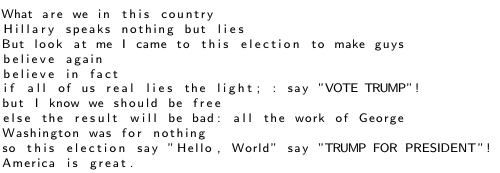
\includegraphics[width=\linewidth,height=0.5\textheight,keepaspectratio]{chapters/04_programming_languages/figures/trump_code.png}
                        \end{figure}
                    \end{column}
                    \begin{column}{0.6\linewidth}
                        \begin{figure}
                            \centering
                            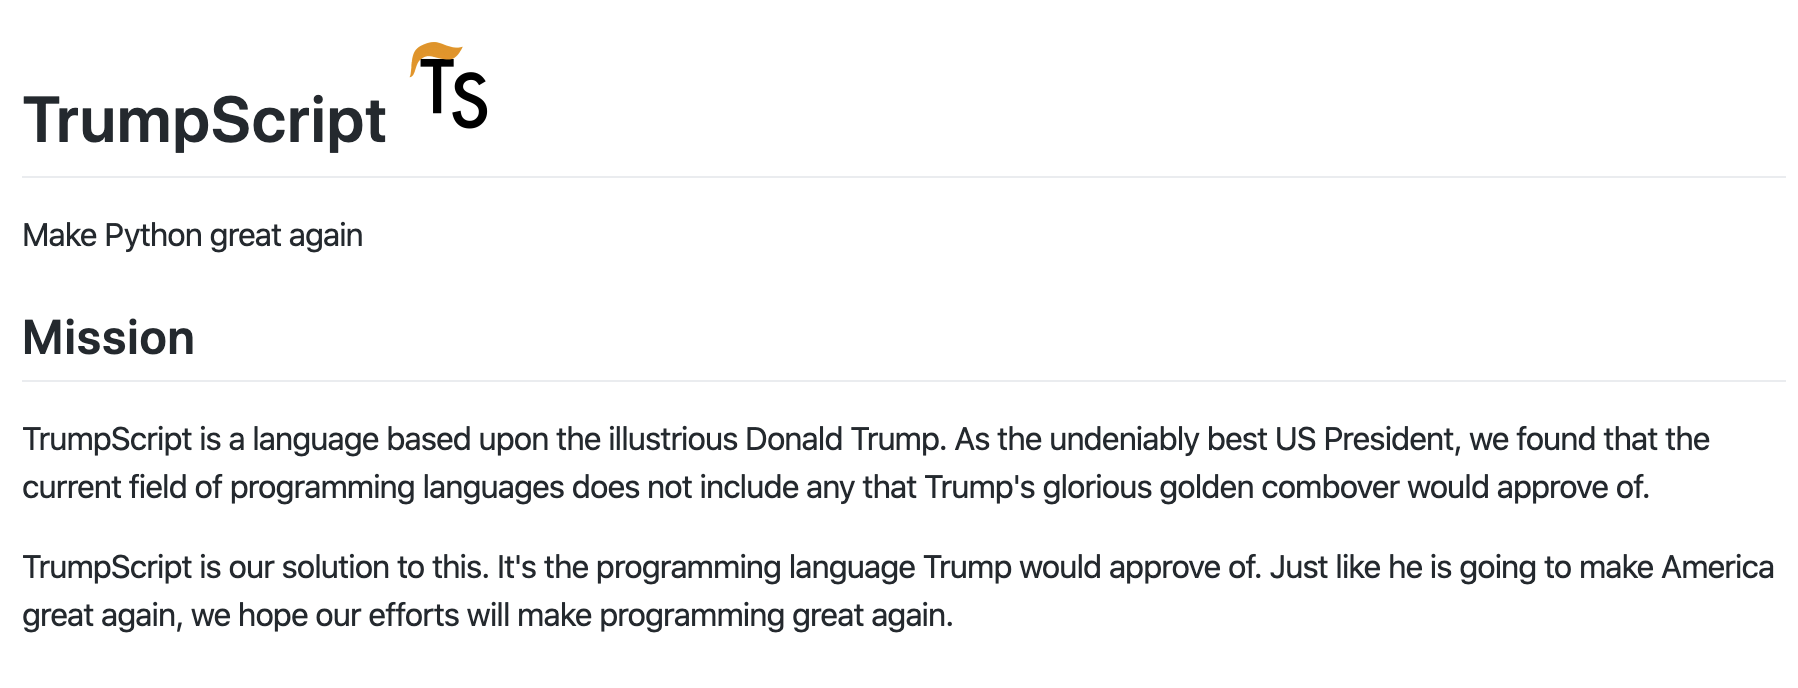
\includegraphics[width=\linewidth,height=0.5\textheight,keepaspectratio]{chapters/04_programming_languages/figures/trump.png}
                            \caption{TrumpScript \cite{trumpscript}}
                        \end{figure}
                    \end{column}
                \end{columns}
                
                \note{\href{https://github.com/samshadwell/TrumpScript}{https://github.com/samshadwell/TrumpScript}}
            \end{frame}
            
            \begin{frame}{Antwort 3: Was hat das mit Programmiersprachen zu tun?}
                \begin{columns}
                    \begin{column}{0.4\linewidth}
                       \begin{figure}
                    \centering
                    
\includegraphics[width=\linewidth,height=0.5\textheight,keepaspectratio]{chapters/04_programming_languages/figures/hello_world_piet.jpg}
                    \caption{\cite{fig:hello_world_piet}}
                \end{figure}
                    \end{column}
                    \begin{column}{0.6\linewidth}
                        \begin{figure}
                            \centering
                            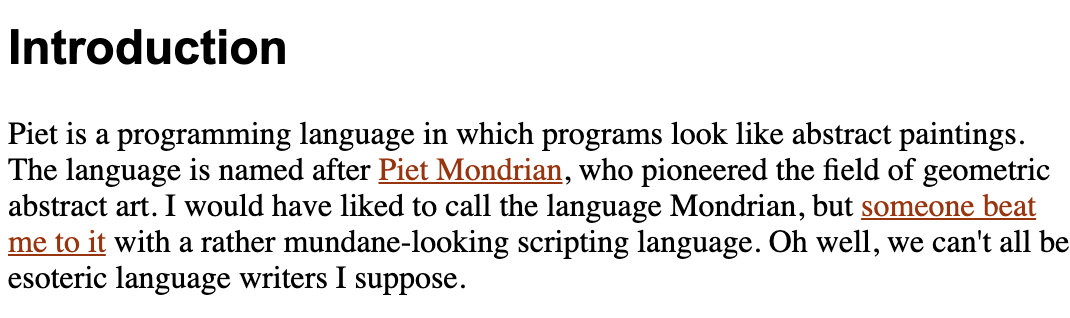
\includegraphics[width=\linewidth,height=0.5\textheight,keepaspectratio]{chapters/04_programming_languages/figures/piet.png}
                            \caption{Piet \cite{piet}}
                        \end{figure}
                    \end{column}
                \end{columns}
                
                \note{
                Code sieht wie ein abstraktes Bild aus \\
                kleinste Einheit: Codel (Code + Pixel) \\
                Werte: Eintreten in schwarzes oder weißes Farbfeld, Zahl der Codels mit zusammenhängender Farbe oder Übergang von einer Farbe zur nächsten
                }
            \end{frame}
        
            
            \begin{frame}{Antwort 4: Was hat das mit Programmiersprachen zu tun?}
                 \lstinputlisting[basicstyle=\tiny]{chapters/04_programming_languages/code/hello_world.bf}
                 
                 \begin{figure}
                            \centering
                            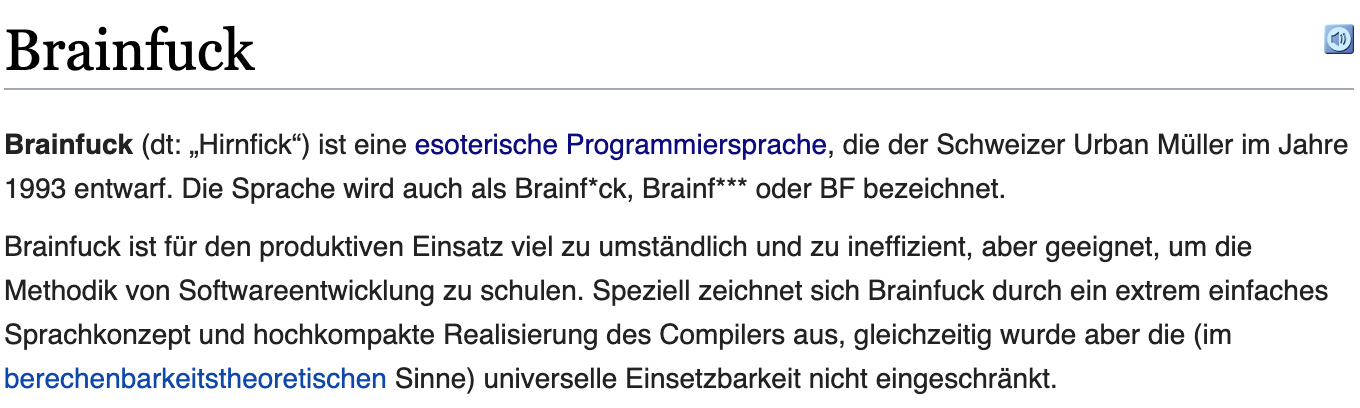
\includegraphics[width=0.7\linewidth,height=0.5\textheight,keepaspectratio]{chapters/04_programming_languages/figures/brainfuck.png}
                            \caption{Brainfuck \cite{brainfuck}}
                \end{figure}
                        
                \note{
                    Jedes Zeichen hat eine unterschiedliche Bedeutung: \\
                    $>$ inkrementiert den Zeiger \\
                    + inkrementiert den aktuellen Zellenwert \\
                    . gibt das aktuelle Zeichen aus
                }
            \end{frame}